\documentclass{capstonedoc}

% Document Info
\title{Sega Genesis Controller Interfacing}
\date{2016-04-02}
\author{Mason Strong, Stephen Just}

\usepackage{cite}
\usepackage[hyphens]{url}

\usepackage{wrapfig}
\usepackage{graphicx}
\graphicspath{ {images/} }

\usepackage{caption}

\begin{document}
\maketitle

%Document body

\begin{wrapfigure}{r}{0.4\textwidth}
  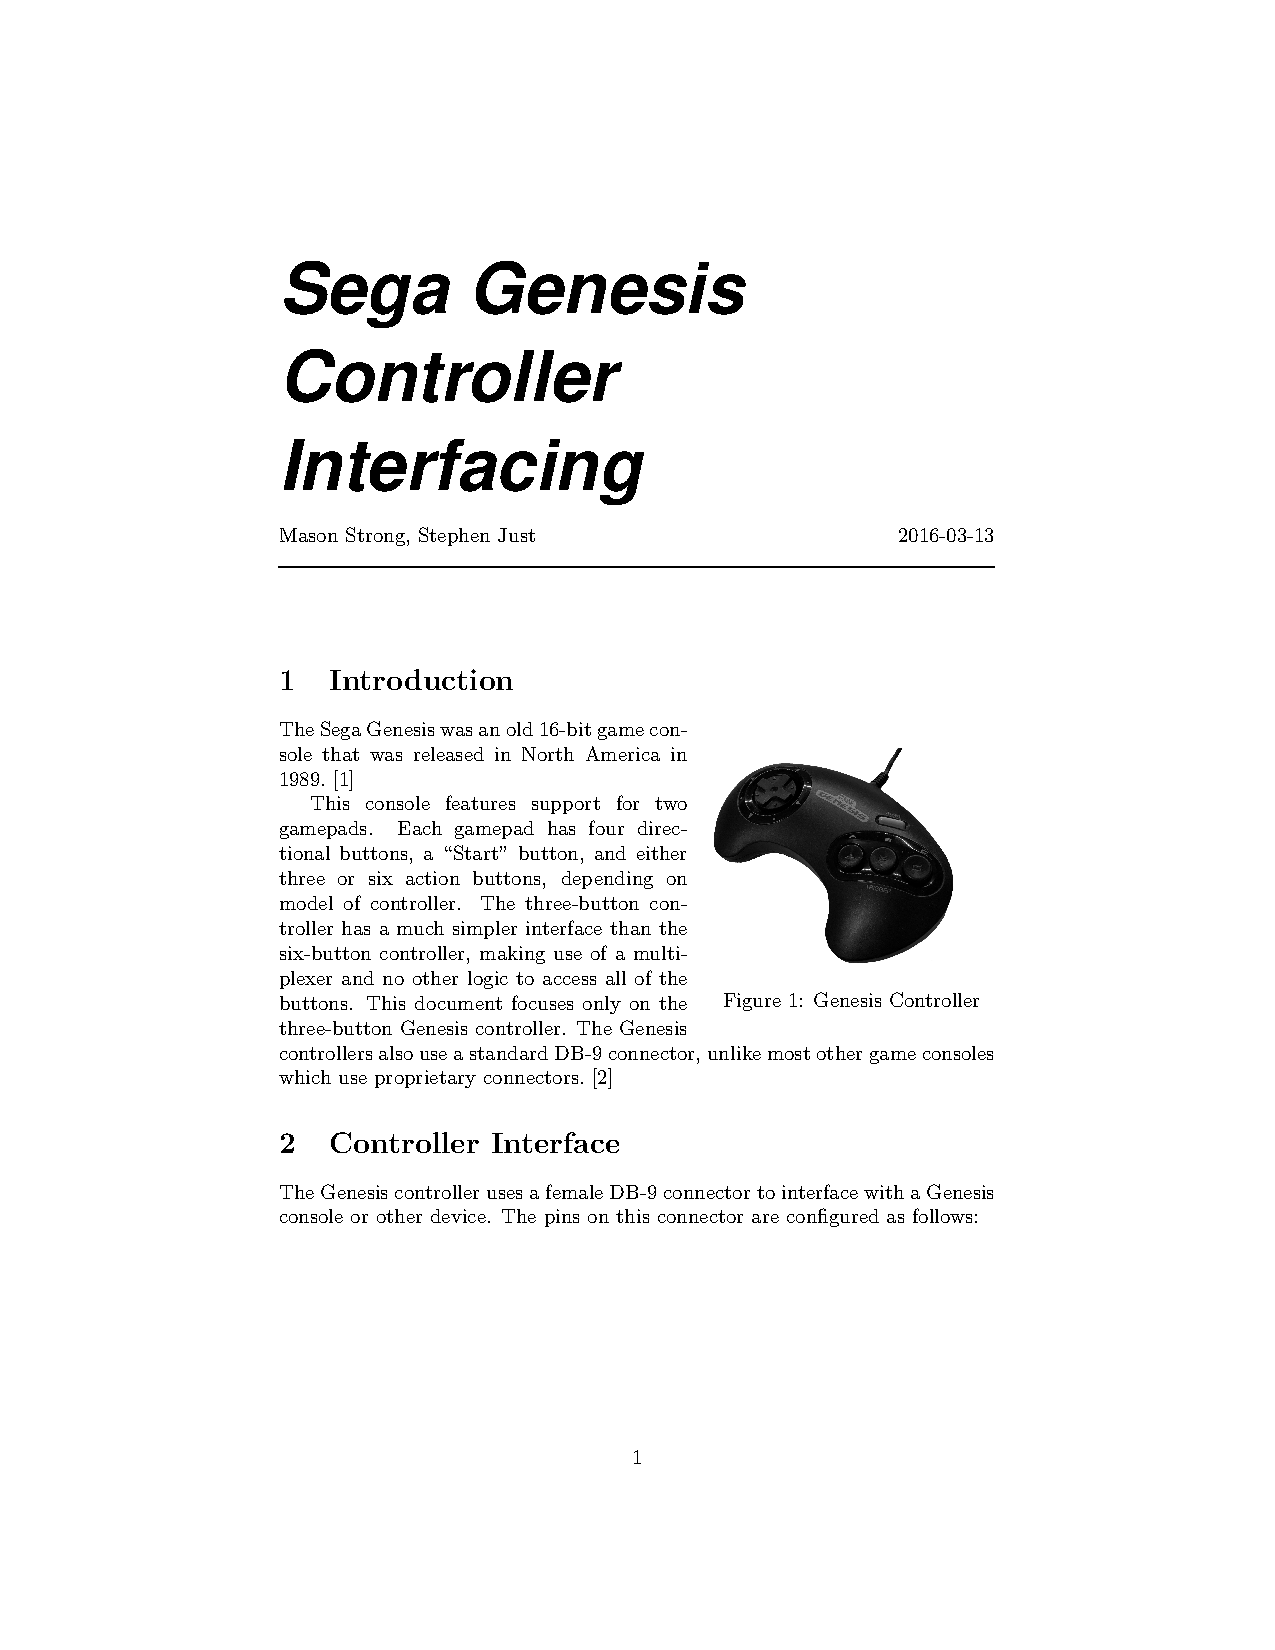
\includegraphics[width=0.35\textwidth]{genesis_controller}
  \caption{Genesis Controller}
  \label{fig:controller_photo}
\end{wrapfigure}

\section{Introduction}
The Sega Genesis was an old 16-bit game console that was released in North
America in 1989. \cite{SGHistory}

This console features support for two gamepads. Each gamepad has four
directional buttons, a ``Start'' button, and either three or six action
buttons, depending on model of controller. The three-button controller has a
much simpler interface than the six-button controller, making use of a
multiplexer and no other logic to access all of the buttons. This document
focuses only on the three-button Genesis controller. The Genesis controllers
also use a standard DB-9 connector, unlike most other game consoles which
use proprietary connectors.\cite{SGCHwInfo}

\section{Controller Interface}
The Genesis controller uses a female DB-9 connector to interface with a Genesis
console or other device. The pins on this connector are configured as follows:

\vspace{5mm}
\begin{tabular}{ l | l | l }
  Pin & Func (select low) & Func (select high) \\ \hline \hline
  1   & up button         & up button          \\
  2   & down button       & down button        \\
  3   & logic low         & left button        \\
  4   & logic low         & right button       \\
  5   & Power (+5 volts)  & Power (+5 Volts)   \\
  6   & A button          & B button           \\
  7   & select signal     & select signal      \\
  8   & Ground            & Ground             \\
  9   & Start button      & C button           \\
\end{tabular}
\vspace{5mm}

While the controller was designed for +5 Volts for power, because of its simple
design, it is possible to determine that it is actually capable of 2 - 6 Volts.
This is possible because the controller only contains a single 74HC157
multiplexer chip inside, whose datasheet specifies that the device is operable
within that range albeit with varying delay times.\cite{TC74HC157AP}

In order to read the buttons on a controller, the master device should apply
a logic high or low to the select pin of the controller, and then query the
state of each of the button pins. Then the master device can switch the state
of the select pin, and then query the values for the other buttons. When a
button is pressed, its value will be logic low. Buttons that are not pressed
will appear as a logic high. Note that reading the up and down buttons of
the controller are not affected by the select signal, as they are connected
directly to the controller plug and not through the multiplexer.

\section{Notes}
On a real Genesis console, the controller's value is read once per video frame,
or 60 times per second. That means that if you are trying to emulate a
controller, the emulated buttons should remain pressed for at least 1/60th of
a second, to ensure that the input is received by the console. Shorter button
presses could be missed entirely.

Be aware that the six-button gamepad has a more complicated interface protocol.
The extra buttons are accessed by toggling the select line on the controller
three times in quick succession. If you want your application to tolerate six-
button controllers, take care not to do this. The six-button controllers should
not go in to this mode if you only toggle the select line once per frame.
This appnote targets the standard three-button genesis controllers and 
corresponding protocol, and the supplied code examples have only been verified
to handle three-button controllers.

To simplify the example project, there is a simple process in the supplied VHDL
top-level file to generate a pulse every 50ms to trigger the Genesis controller
block, as opposed to connecting the block to a VSync signal.

\section{System Requirements}

\subsection{Hardware}

Ensure that you are in possession of a three-button genesis controller, and a 
corresponding adapter board to interface the DB9 connector with the appropriate 
GPIO pins on the DE2. Should an adapter board be unavailable, a 40-pin header 
can be connected to two male DB9 connectors on a breadboard using the pinout
described by the schematic in Figure~\ref{fig:schematic}. Then, you can use a
ribbon cable to connect your breadboard to your DE2.

\begin{figure}[h]
  \centering
  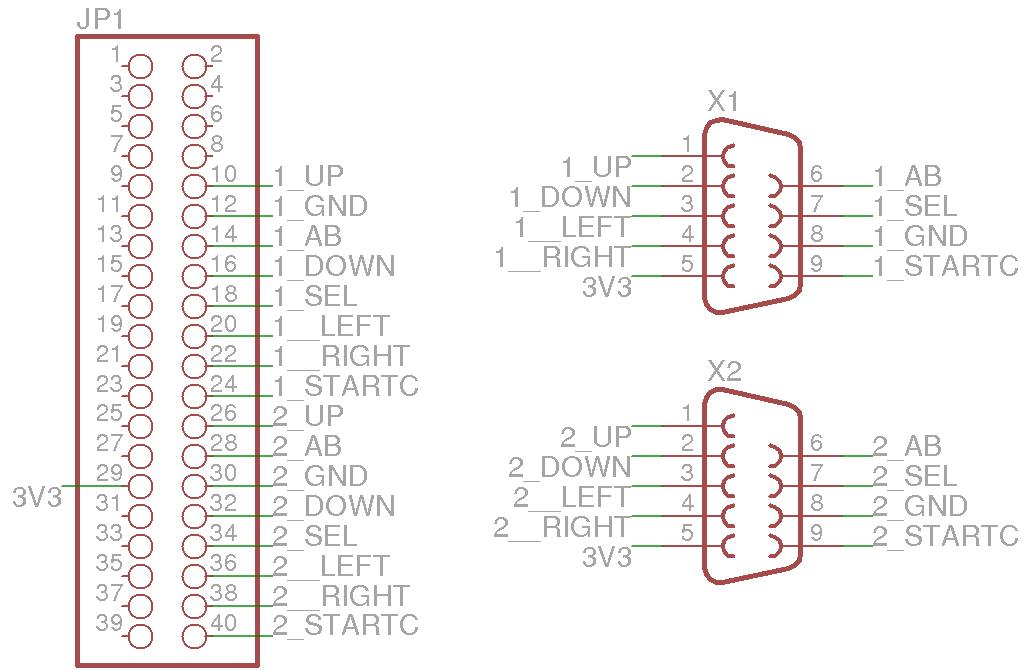
\includegraphics[width=7cm]{schematic}
  \caption{Connection Schematic}
  \label{fig:schematic}
\end{figure}

An Eagle project with a custom PCB design is included in
\texttt{pcb\_design.tar.gz}, found with this document.

\subsection{Qsys}

In order to interface with Genesis controllers, you may use the Qsys-compatible
IP Core supplied with the example code in the \texttt{ip} directory. This IP
core is also available standalone in the \texttt{genesis\_ipcore.tar.gz} archive
supplied with this document.

With the Genesis IP Core included in your project, you can connect it to your
Qsys system. Figure~\ref{fig:qsys_system} shows how the Genesis Controller
Interface can be connected to your system.

\begin{figure}[h]
  \centering
  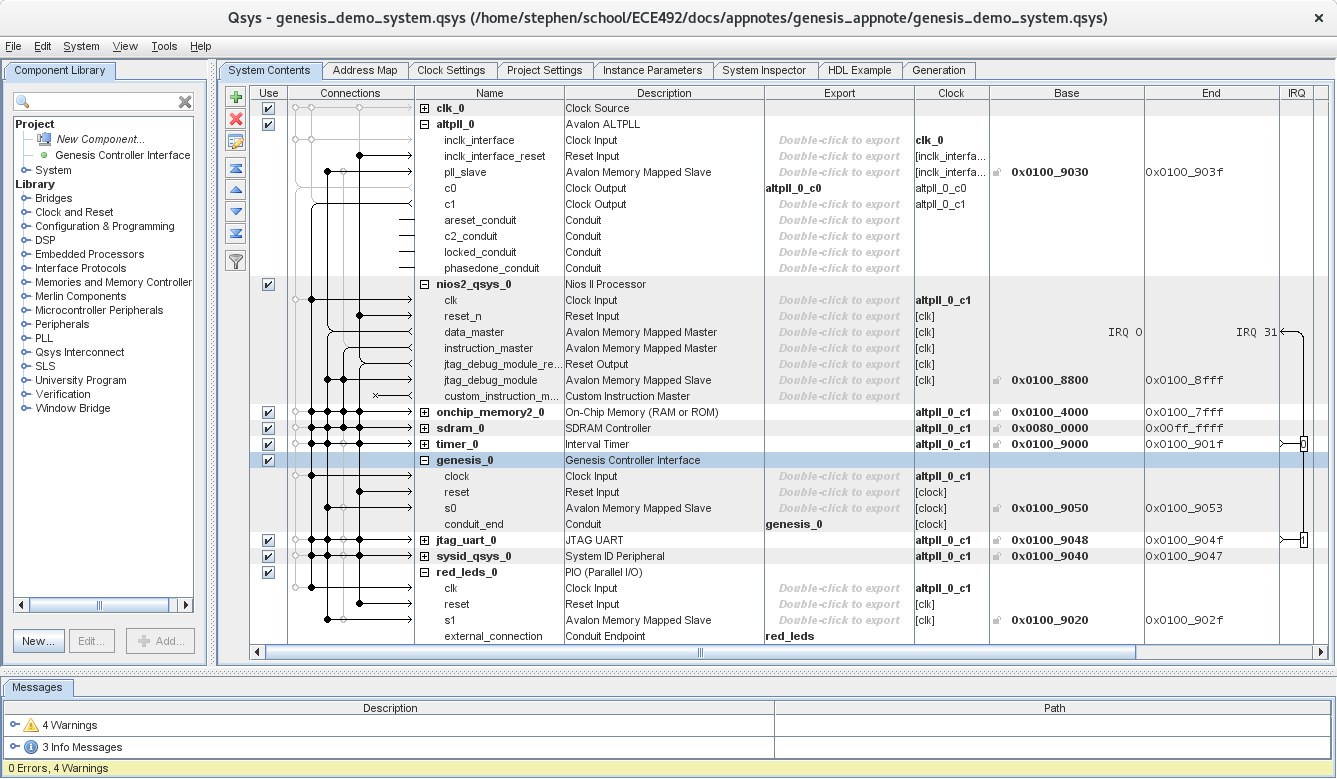
\includegraphics[width=\textwidth]{qsys_system}
  \caption{Qsys System Connections}
  \label{fig:qsys_system}
\end{figure}

\subsection{Quartus}

The Genesis controllers are connected to the DE2 via one of the GPIO ports. In
our system, we used \texttt{GPIO\_1}. To ensure correct controller behaviour,
the GPIO connector should be configured as high-impedance by default, as is
shown in Listing~\ref{lst:tl_port}.

As well, the FPGA's internal weak pull-up resistors should be enabled to ensure
that the inputs are not floating when controllers are not plugged in to the
system. This can be done by adding the lines in Listing~\ref{lst:qsf_pullup} to
your project's QSF file.

\noindent\begin{minipage}{\textwidth}
\begin{lstlisting}[language={vhdl},caption={Entity for Top-Level},label={lst:tl_port}]
entity genesis_demo is
	port
	(
		-- Clocks
		CLOCK_50     : in       std_logic;

		-- SDRAM on board
		DRAM_ADDR    : out      std_logic_vector (11 downto 0);
		DRAM_BA_0    : out      std_logic;
		DRAM_BA_1    : out      std_logic;
		DRAM_CAS_N   : out      std_logic;
		DRAM_CKE     : out      std_logic;
		DRAM_CLK     : out      std_logic;
		DRAM_CS_N    : out      std_logic;
		DRAM_DQ      : inout    std_logic_vector (15 downto 0);
		DRAM_LDQM    : out      std_logic;
		DRAM_UDQM    : out      std_logic;
		DRAM_RAS_N   : out      std_logic;
		DRAM_WE_N    : out      std_logic;

		-- Input switches and buttons
		KEY           : in       std_logic_vector (3 downto 0);

		-- Indicator LEDs
		LEDR         : out      std_logic_vector (17 downto 0);

		-- GPIO Port 1
		GPIO_1 : inout std_logic_vector (35 downto 0) := (others => 'Z')
	);
end genesis_demo;
\end{lstlisting}
\end{minipage}

\begin{lstlisting}[language={tcl},caption={Commands to Enable GPIO Pull-Up Resistors},label={lst:qsf_pullup}]
set_instance_assignment -name WEAK_PULL_UP_RESISTOR ON -to GPIO_1[0]
set_instance_assignment -name WEAK_PULL_UP_RESISTOR ON -to GPIO_1[1]
set_instance_assignment -name WEAK_PULL_UP_RESISTOR ON -to GPIO_1[2]
set_instance_assignment -name WEAK_PULL_UP_RESISTOR ON -to GPIO_1[3]
set_instance_assignment -name WEAK_PULL_UP_RESISTOR ON -to GPIO_1[4]
set_instance_assignment -name WEAK_PULL_UP_RESISTOR ON -to GPIO_1[5]
set_instance_assignment -name WEAK_PULL_UP_RESISTOR ON -to GPIO_1[6]
set_instance_assignment -name WEAK_PULL_UP_RESISTOR ON -to GPIO_1[7]
set_instance_assignment -name WEAK_PULL_UP_RESISTOR ON -to GPIO_1[8]
set_instance_assignment -name WEAK_PULL_UP_RESISTOR ON -to GPIO_1[9]
set_instance_assignment -name WEAK_PULL_UP_RESISTOR ON -to GPIO_1[10]
set_instance_assignment -name WEAK_PULL_UP_RESISTOR ON -to GPIO_1[11]
set_instance_assignment -name WEAK_PULL_UP_RESISTOR ON -to GPIO_1[12]
set_instance_assignment -name WEAK_PULL_UP_RESISTOR ON -to GPIO_1[13]
set_instance_assignment -name WEAK_PULL_UP_RESISTOR ON -to GPIO_1[14]
set_instance_assignment -name WEAK_PULL_UP_RESISTOR ON -to GPIO_1[15]
set_instance_assignment -name WEAK_PULL_UP_RESISTOR ON -to GPIO_1[16]
set_instance_assignment -name WEAK_PULL_UP_RESISTOR ON -to GPIO_1[17]
set_instance_assignment -name WEAK_PULL_UP_RESISTOR ON -to GPIO_1[18]
set_instance_assignment -name WEAK_PULL_UP_RESISTOR ON -to GPIO_1[19]
set_instance_assignment -name WEAK_PULL_UP_RESISTOR ON -to GPIO_1[20]
set_instance_assignment -name WEAK_PULL_UP_RESISTOR ON -to GPIO_1[21]
set_instance_assignment -name WEAK_PULL_UP_RESISTOR ON -to GPIO_1[22]
set_instance_assignment -name WEAK_PULL_UP_RESISTOR ON -to GPIO_1[23]
set_instance_assignment -name WEAK_PULL_UP_RESISTOR ON -to GPIO_1[24]
set_instance_assignment -name WEAK_PULL_UP_RESISTOR ON -to GPIO_1[25]
set_instance_assignment -name WEAK_PULL_UP_RESISTOR ON -to GPIO_1[26]
set_instance_assignment -name WEAK_PULL_UP_RESISTOR ON -to GPIO_1[27]
set_instance_assignment -name WEAK_PULL_UP_RESISTOR ON -to GPIO_1[28]
set_instance_assignment -name WEAK_PULL_UP_RESISTOR ON -to GPIO_1[29]
set_instance_assignment -name WEAK_PULL_UP_RESISTOR ON -to GPIO_1[30]
set_instance_assignment -name WEAK_PULL_UP_RESISTOR ON -to GPIO_1[31]
set_instance_assignment -name WEAK_PULL_UP_RESISTOR ON -to GPIO_1[32]
set_instance_assignment -name WEAK_PULL_UP_RESISTOR ON -to GPIO_1[33]
set_instance_assignment -name WEAK_PULL_UP_RESISTOR ON -to GPIO_1[34]
set_instance_assignment -name WEAK_PULL_UP_RESISTOR ON -to GPIO_1[35]
\end{lstlisting}

The Qsys system containing the Genesis controller interface component includes
the ports similar to the ones shown in Listing~\ref{lst:comp_port} within its
component declaration.

\begin{lstlisting}[language={vhdl},caption={Qsys System Ports for Genesis Controller},label={lst:comp_port}]
genesis_0_trigger                   : in    std_logic   := 'X';
genesis_0_dpad_up_input1            : in    std_logic   := 'X';
genesis_0_dpad_down_input1          : in    std_logic   := 'X';
genesis_0_dpad_left_input1          : in    std_logic   := 'X';
genesis_0_dpad_right_input1         : in    std_logic   := 'X';
genesis_0_select_input1             : out   std_logic;
genesis_0_start_c_input1            : in    std_logic  := 'X';
genesis_0_ab_input1                 : in    std_logic  := 'X';
genesis_0_dpad_up_input2            : in    std_logic  := 'X';
genesis_0_dpad_down_input2          : in    std_logic  := 'X';
genesis_0_dpad_left_input2          : in    std_logic  := 'X';
genesis_0_dpad_right_input2         : in    std_logic  := 'X';
genesis_0_select_input2             : out   std_logic;
genesis_0_start_c_input2            : in    std_logic  := 'X';
genesis_0_ab_input2                 : in    std_logic  := 'X';
\end{lstlisting}

The instance of the Qsys system defines which pins on the DE2's GPIO header are
connected to the pins on the Genesis controllers. The configuration used for our
interface PCB is shown in Listing~\ref{lst:port_map}.

\begin{lstlisting}[language={vhdl},caption={Port Map Configuration},label={lst:port_map}]
genesis_0_trigger                       => genesis_poll_trigger,
genesis_0_dpad_up_input1                => GPIO_1(35),
genesis_0_dpad_down_input1              => GPIO_1(31),
genesis_0_dpad_left_input1              => GPIO_1(27),
genesis_0_dpad_right_input1             => GPIO_1(25),
genesis_0_select_input1                 => GPIO_1(29),
genesis_0_start_c_input1                => GPIO_1(23),
genesis_0_ab_input1                     => GPIO_1(33),
genesis_0_dpad_up_input2                => GPIO_1(13),
genesis_0_dpad_down_input2              => GPIO_1(9),
genesis_0_dpad_left_input2              => GPIO_1(5),
genesis_0_dpad_right_input2             => GPIO_1(3),
genesis_0_select_input2                 => GPIO_1(7),
genesis_0_start_c_input2                => GPIO_1(1),
genesis_0_ab_input2                     => GPIO_1(11),
\end{lstlisting}

\subsection{Nios II SBT}

A sample project is included in the companion code to read the Genesis
controllers connected to the system, and output to the red LEDs on the DE2.
This is located in the \texttt{software} directory of the companion code
package. Import the project and its BSP into a new workspace.

\section{C Driver API}

A driver is provided with the Genesis IP Core. To make use of this driver,
include \texttt{genesis.h} into your project. \texttt{genesis.h} is
automatically added to your BSP when you include the Genesis IP Core in your
system. Listing~\ref{lst:c_example} provides an example of how you might read
the state of two Genesis controllers in software.

\begin{lstlisting}[language=c,tabsize=2,caption={Reading Genesis Controller Example},label={lst:c_example}]
#include <stdio.h>
#include <system.h>
#include <genesis.h>

int main(void)
{
	// Initialize the Genesis controller interface
	genesis_open_dev(GENESIS_0_NAME);

	genesis_controller_t player1, player2;
	while (1)
	{
		// Poll the status of each Genesis controller
		player1 = genesis_get(GENESIS_PLAYER_1);
		player2 = genesis_get(GENESIS_PLAYER_2);

		// Check which buttons are pressed on controller 1
		if (player1.up){
			printf("1 Up was pressed\n");
		}
		if (player1.down){
			printf("1 Down was pressed\n");
		}
		if (player1.left){
			printf("1 Left was pressed\n");
		}
		if (player1.right){
			printf("1 Right was pressed\n");
		}
		if (player1.a){
			printf("1 A was pressed\n");
		}
		if (player1.b){
			printf("1 B was pressed\n");
		}
		if (player1.c){
			printf("1 C was pressed\n");
		}
		if (player1.start){
			printf("1 Start was pressed\n");
		}

		// Check which buttons are pressed on controller 2
		if (player2.up){
			printf("2 Up was pressed\n");
		}
		if (player2.down){
			printf("2 Down was pressed\n");
		}
		if (player2.left){
			printf("2 Left was pressed\n");
		}
		if (player2.right){
			printf("2 Right was pressed\n");
		}
		if (player2.a){
			printf("2 A was pressed\n");
		}
		if (player2.b){
			printf("2 B was pressed\n");
		}
		if (player2.c){
			printf("2 C was pressed\n");
		}
		if (player2.start){
			printf("2 Start was pressed\n");
		}
    }

	return 0;
}
\end{lstlisting}

\newpage

% References
\bibliographystyle{ieeetr}
\bibliography{genesis_controller}

\end{document}
